\section{Cross-dataset collapse and its diagnosis}
\label{sec:analysis}

\subsection{The collapse (answering RQ2)}
Evaluated unchanged on the three external sets under the binary alignment of \cref{tab:mapping},
the student's accuracy falls from $0.966$ internally to $0.639$ (\herlev), $0.605$ (\hicervix) and
$0.532$ (\apacc)---a $33$-to-$43$-point drop (\herlev\ $33$, \hicervix\ $36$, \apacc\ $43$) that
\emph{supports} \textbf{H2} (\cref{tab:cross}, \cref{fig:cmcross}). Threshold-free AUROC tells the
same story more cleanly: $0.728$, $0.594$, $0.525$. Two observations sharpen the result. First, on
\herlev\ and \hicervix\ the accuracy at $\tau{=}0.5$ is \emph{below the majority-class baseline}
($0.639\!<\!0.74$; $0.605\!<\!0.621$, the latter only a razor-thin $1.6$-point gap): a model that
always predicted the majority class would score at least as well. Second, the error structure differs
by dataset---the model over-predicts \emph{abnormal} on \apacc\ (specificity $0.417$) and
\emph{normal} on \hicervix\ (sensitivity $0.386$, missing most abnormal cells). A single global
threshold is clearly mis-placed for each domain.

\begin{table*}[tb]
\caption{\textbf{Cross-dataset binary results (student).} Internal \sipakmed\ accuracy is $0.966$.
ECE is the binary expected calibration error ($15$ bins; in-distribution binary ECE is $0.008$);
$\Delta P$ is the separation between mean $\pabn$ on true-abnormal vs.\ true-normal cells (positive
$=$ correct ordering); ``Maj.'' is the majority-class baseline. At $\tau{=}0.5$, accuracy falls
\emph{below} the majority baseline for \herlev\ and \hicervix\ despite AUROC$>0.5$, and ECE is
$27\!-\!41\times$ the internal value.}
\label{tab:cross}
\centering\small
\begin{tabular}{@{}lccccccccc@{}}
\toprule
Dataset & $n$ & Acc & Bal.\ acc & Sens & Spec & AUROC & ECE & $\Delta P$ & Maj. \\
\midrule
\herlev   & 917  & 0.639 & 0.651 & 0.625 & 0.678 & \best{0.728} & 0.256 & $+0.284$ & 0.74 \\
\hicervix & 4823 & 0.605 & 0.562 & 0.386 & 0.738 & 0.594 & 0.219 & $+0.112$ & 0.62 \\
\apacc    & 1125 & 0.532 & 0.535 & 0.654 & 0.417 & 0.525 & 0.328 & $+0.045$ & 0.51 \\
\midrule
\multicolumn{10}{@{}l}{\footnotesize Internal \sipakmed: Acc $0.966$, binary ECE $0.008$. \quad Higher ECE $=$ worse calibration.}\\
\bottomrule
\end{tabular}
\end{table*}

\begin{figure*}[tb]
  \centering
  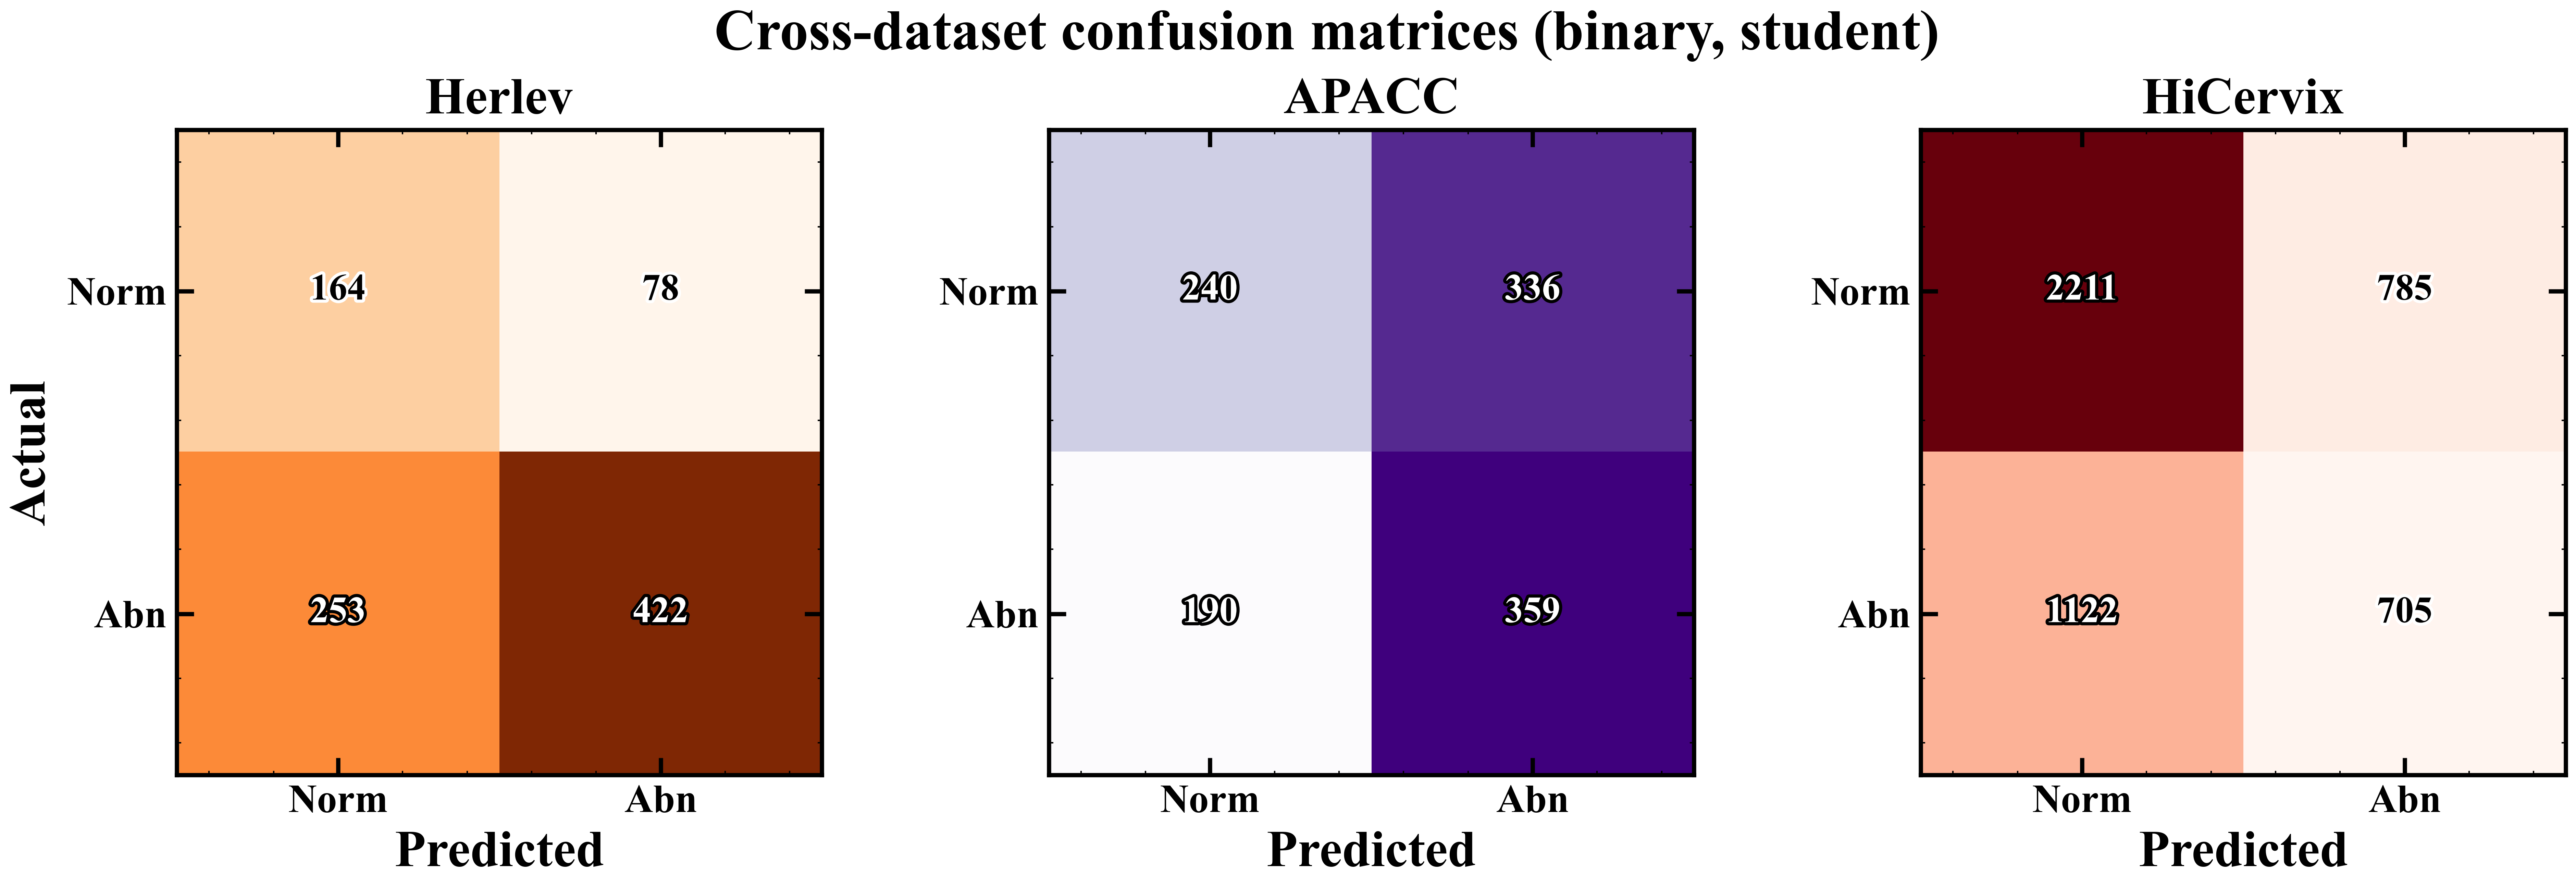
\includegraphics[width=\textwidth]{cm_cross_combined.png}
  \caption{\textbf{Cross-dataset confusion matrices (binary, student).} The model over-predicts
  \emph{abnormal} on \apacc\ (low specificity) and \emph{normal} on \hicervix\ (low sensitivity).}
  \label{fig:cmcross}
\end{figure*}

\subsection{It is not a labelling artefact (answering RQ3)}
The decisive question is whether this collapse is an artefact of our binary crosswalk. It is not. If
the mapping were flipped or mis-defined, the decision score $\pabn$ would rank abnormal cells
\emph{below} normal ones and AUROC would fall \emph{below} $0.5$. The opposite holds in every dataset:
the class-conditional separation $\Delta P=\overline{\pabn}_{\text{abn}}-\overline{\pabn}_{\text{norm}}$
is \emph{positive everywhere} ($+0.284$ \herlev, $+0.112$ \hicervix, $+0.045$ \apacc; \cref{fig:sep},
\cref{tab:cross}) and every AUROC exceeds chance. The score is correctly oriented---the model knows,
weakly, which cells are abnormal---so the labels are not the problem. We additionally audited each
per-dataset mapper against the native taxonomies (\cref{tab:mapping}); the stricter \herlev-columnar
variant shifts the headline by $<\!1$ point. \textbf{H3 is supported}: the failure is genuine, not an
alignment artefact.

\begin{figure*}[tb]
  \centering
  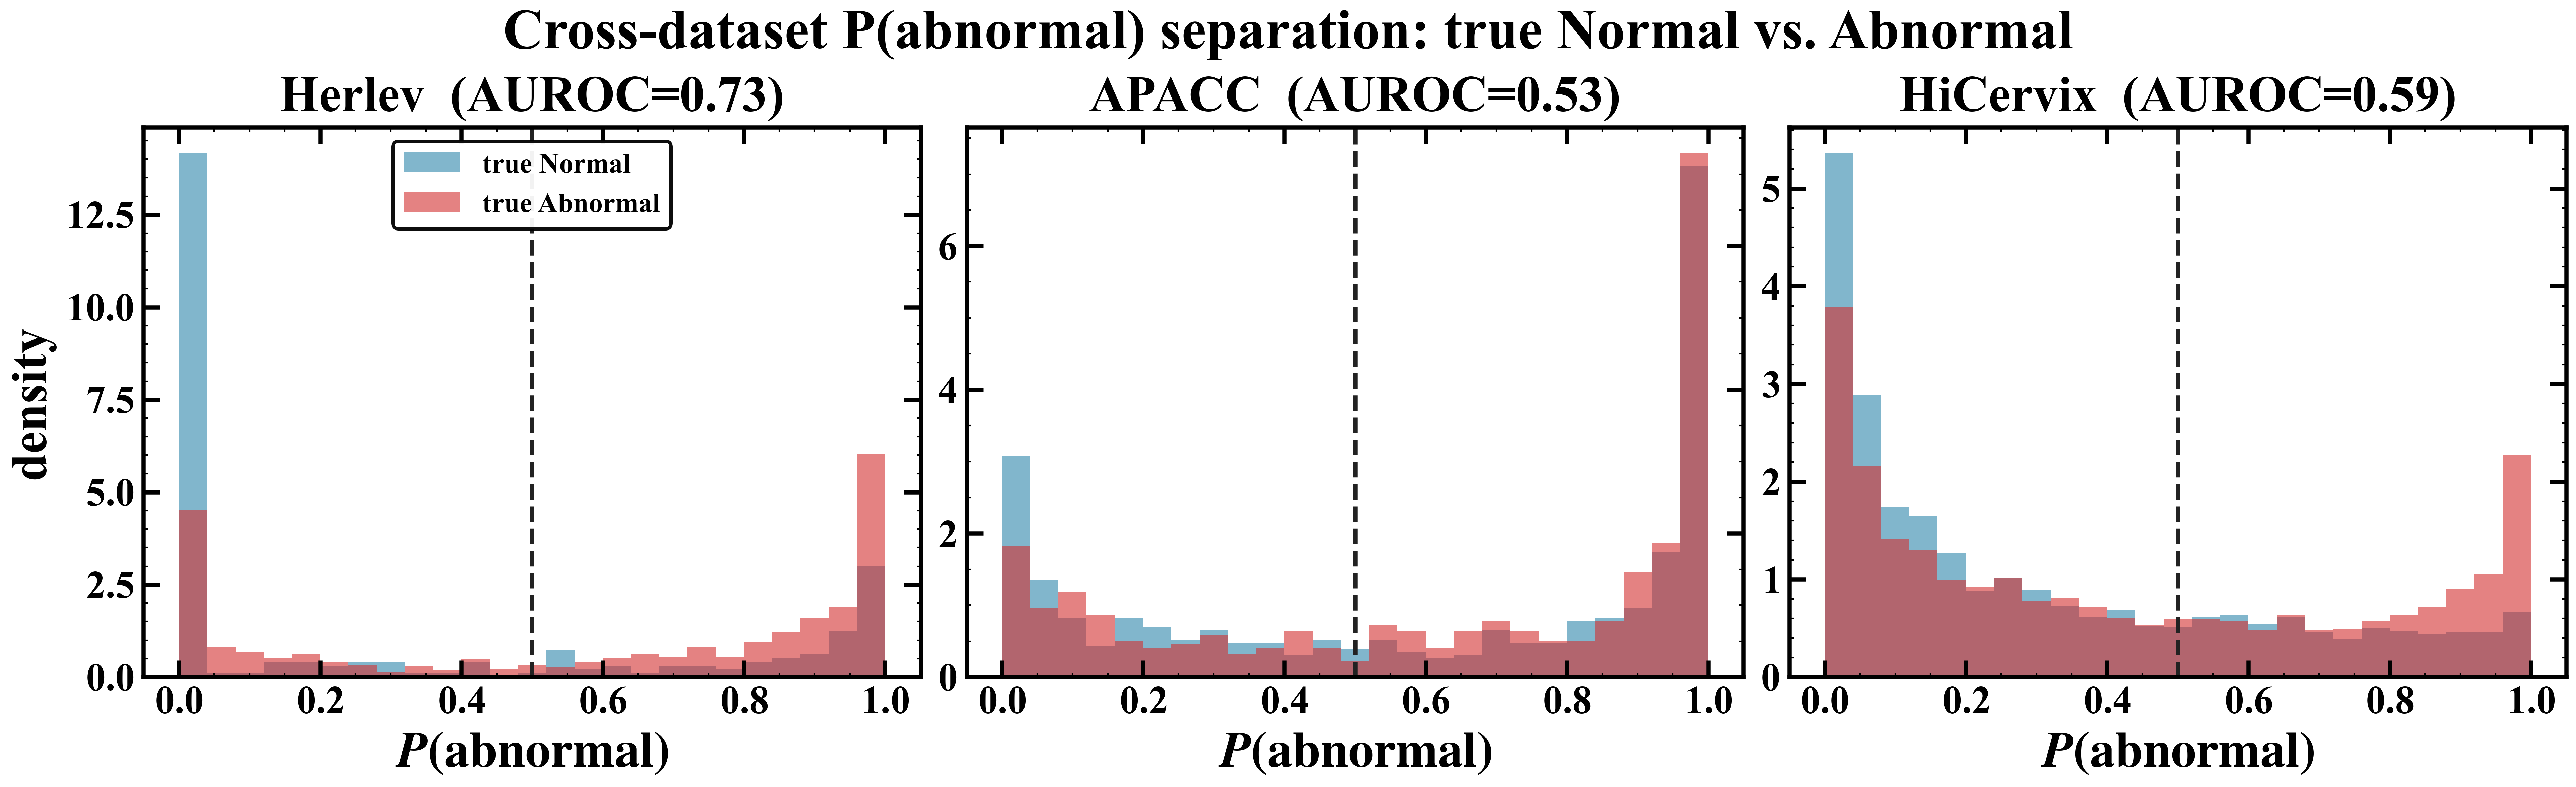
\includegraphics[width=\textwidth]{cross_separation.png}
  \caption{\textbf{$\pabn$ separation.} Distribution of the decision score for true-normal (blue) vs.\
  true-abnormal (red) cells. Separation is clear on \herlev\ (AUROC $0.73$), weak on \hicervix\
  ($0.59$) and essentially absent on \apacc\ ($0.53$). The dashed line is $\tau{=}0.5$; a flipped label
  map would swap the colours and push AUROC below $0.5$.}
  \label{fig:sep}
\end{figure*}

\subsection{What actually breaks}
Three mechanisms, jointly, explain the numbers.

\noindent\textbf{(1) Operating-point miscalibration that does not transfer.} The in-distribution
confidence is well calibrated (binary ECE $0.008$), but this property is \emph{domain-local}: external
binary ECE balloons to $0.256$ (\herlev), $0.219$ (\hicervix) and $0.328$ (\apacc)---a
$27\!-\!41\times$ increase over the internal value (\cref{tab:cross}). The $\pabn$ distribution shifts
wholesale per domain---mean $\pabn$ is $0.61$ on \apacc\ (vs.\ a base abnormal rate of $0.49$, hence
over-calling abnormal) and $0.35$ on \hicervix\ (vs.\ $0.38$, hence under-calling)---so the fixed
$\tau{=}0.5$ lands in the wrong place and discards the ranking signal that AUROC shows is present.
This is exactly why accuracy can fall \emph{below} the majority baseline while AUROC stays above
chance. Quantifying the gap, a per-dataset \emph{oracle} threshold (chosen on the test set, reported
only to bound the calibration loss) recovers accuracy to $0.75$ (\herlev, $\tau{=}0.05$) and $0.65$
(\hicervix, $\tau{=}0.85$)---but not \apacc\ ($0.53$), which has no signal to recover. The
non-transfer of calibration is the cross-dataset half of \textbf{H4}.

\noindent\textbf{(2) Signal degrades with slide-preparation distance.} The retained AUROC is ordered
by how far each dataset's preparation sits from \sipakmed's conventional smear:
\herlev\ (conventional) $0.73$ $>$ \hicervix\ (liquid-based) $0.59$ $>$ \apacc\ (auto-segmented noisy
crops) $0.53\!\approx\!$ chance. The model has, in effect, learned features entangled with the
preparation pipeline---a cytology instance of shortcut learning~\cite{geirhos2020shortcut}---and the
discriminative signal erodes monotonically as that pipeline diverges.

\noindent\textbf{(3) The internal number is itself optimistic.} The $0.966$ is measured on a random
per-cell split, which places cells from the \emph{same} field-of-view into both train and validation;
those cells share staining, focus and debris, so the validation estimate is inflated by leakage. A
leakage-safe, cluster-grouped split (no field-of-view shared across partitions) would lower it,
widening the true internal-to-external gap beyond the $33\!-\!43$ points measured here. The honest
headline is therefore worse than even \cref{tab:cross} suggests.
